\section{Transport Protocols and Mobility Choices for ABR Streaming: Performance vs Energy Efficiency}
Any ABR take decision based on the directly or indirectly observed network throughput. However, this throughput is highly depends on the underlying transport protocol QUIC or TCP. As all the ABR algorithms are primarily designed with TCP in the mind, we want to know if those existing ABR algorithm can work fine with the QUIC or other set of algorithms are required. On the other hand, the performance of an ABR algorithm can indirectly impact the power consumption of smartphones due to the nature of the radio resource controller (RRC).

\subsection{TCP vs QUIC: YouTube}
YouTube started using QUIC as an alternative to TCP via Google chrome and chromium browser. Both of these browser support flag to enable or disable QUIC during run time. So we run player ~175 videos by enabling and disabling the QUIC and record the HAR and {\tt tcpdump} trace. 
\subsubsection{Observation}
We want to know QUIC provide better quality than TCP or not. So, we look for the three parameters rebuffering, average quality and quality switches in our collected traces. We find that QUIC incurs less quality switches than TCP and over all quality is better with QUIC than the TCP. In terms of rebuffering we find interesting results. When network quality is very poor, QUIC suffers more than the TCP. However, TCP suffers more when network quality is better.

\subsection{TCP vs QUIC: DASH}
We compare performance of modern ABRs like BOLA, MPC, and Pensieve between QUIC and TCP. For the experiment purpose, we use the open source DASH-IF player and publicly available network trace to throttle the connection with the help of {\tt mahimahi} tool. We keep the server and the experimental client in the same network and throttle the connection using {\tt mahimahi}. In this experiment we played approx 50 videos of total 45 hours playback time using various ABR algorithm.

\subsubsection{Observation}
Our initial observations showed that the QUIC is performing poorly for all most all the scenarios in term of all the QoE components and the over all QoE for most of the scenarios. Fig.~\ref{fig:chap03s2:RebufferTime_n} and Fig.~\ref{fig:chap03s2:QOE_n} depict the observations on rebuffering and QoE.
\begin{figure*}[!h]
%	\begin{minipage}[t]{0.48\linewidth}
%		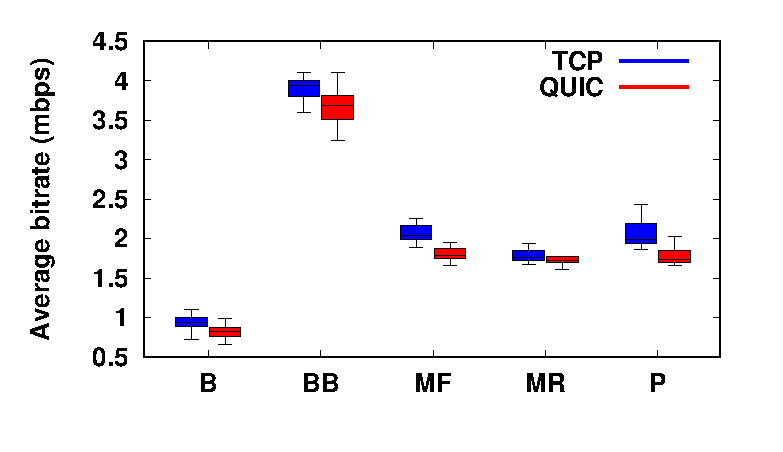
\includegraphics[width=\linewidth]{img/QUIC/bitrate_box}
%		\caption{\label{fig:chap03s2:averageQuality_n}Average Playback Video Quality for Different ABR Techniques ($p<0.05$ for all the metrics)}
%	\end{minipage}\hfill
%	\begin{minipage}[t]{0.48\linewidth}
%		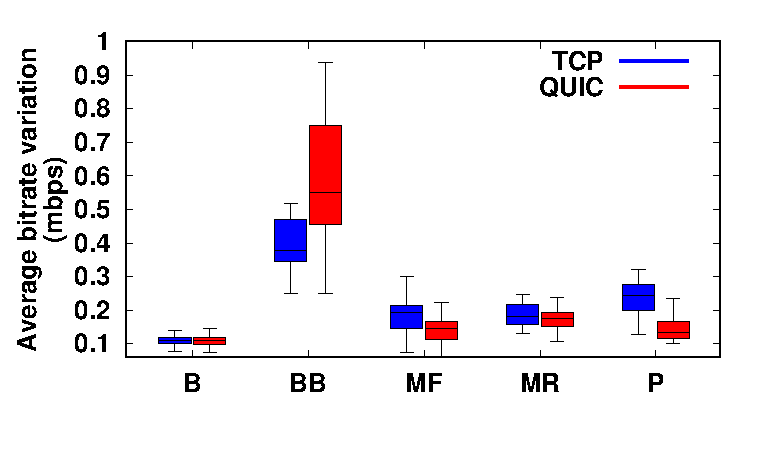
\includegraphics[width=\linewidth]{img/QUIC/smooth_box}
%		\caption{\label{fig:chap03s2:averageQualityVariation_n}Average Playback Quality Variation for Different ABR Techniques ($p<0.05$ for all the metrics except BOLA and MPC-Robust)}
%	\end{minipage}
%	
	\begin{minipage}[t]{0.48\linewidth}
		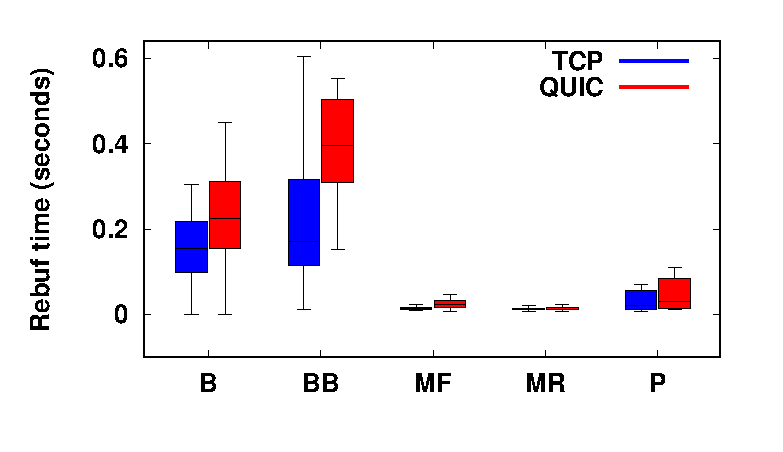
\includegraphics[width=\linewidth]{img/QUIC/rebuf_box}
		\caption{\label{fig:chap03s2:RebufferTime_n}Rebuffering Time for Different ABR Techniques ($p<0.05$ for all the metrics except Pensieve and MPC-Robust)}
	\end{minipage}\hfill
	\begin{minipage}[t]{0.48\linewidth}
		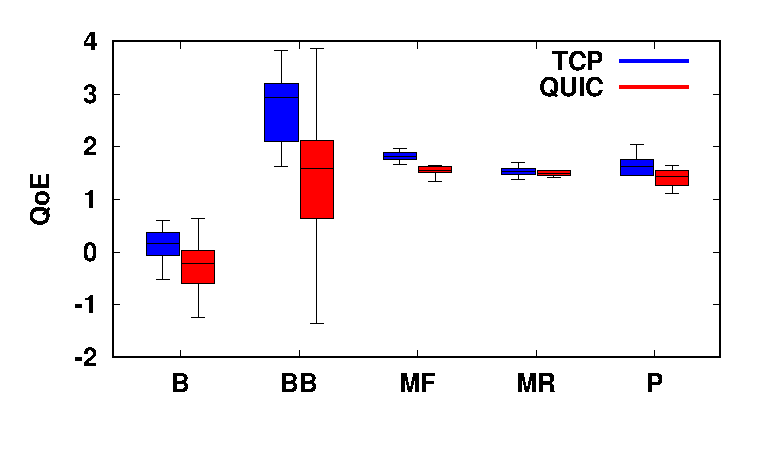
\includegraphics[width=\linewidth]{img/QUIC/qoe_box}
		\caption{\label{fig:chap03s2:QOE_n}Overall QoE for Different ABR Techniques ($p<0.05$ for all the metrics except MPC-Robust)}
	\end{minipage}
\end{figure*}

\subsection{Energy Consumption due to ABR Streaming: An Ex- perimental Analysis}
